\documentclass[12pt, twocolumn]{article}

% 引入相关的包
\usepackage{amsmath, listings, fontspec, geometry, graphicx, ctex, color, subfigure}

% 设定页面的尺寸和比例
\geometry{left = 1.5cm, right = 1.5cm, top = 1.5cm, bottom = 1.5cm}

% 设定两栏之间的间距
\setlength\columnsep{1cm}

% 设定字体,为代码的插入作准备
\newfontfamily\ubuntu{Ubuntu Mono}

% 头部信息
\title{\normf{这是标题}}
\author{\normf{陈烁龙}}
\date{\normf{\today}}

% 代码块的风格设定
\lstset{
	language=C++,
	basicstyle=\scriptsize\ubuntu,
	keywordstyle=\textbf,
	stringstyle=\itshape,
	commentstyle=\itshape,
	numberstyle=\scriptsize\ubuntu,
	showstringspaces=false,
	numbers=left,
	numbersep=8pt,
	tabsize=2,
	frame=single,
	framerule=1pt,
	columns=fullflexible,
	breaklines,
	frame=shadowbox, 
	backgroundcolor=\color[rgb]{0.97,0.97,0.97}
}

% 字体族的定义
\newcommand{\normf}{\kaishu}
\newcommand{\boldf}{\heiti}
\newcommand\keywords[1]{\boldf{关键词:} \normf #1}
\newcommand{\lieal[1]}{\left\lfloor #1 \right\rfloor_\times}

\begin{document}
	
	% 插入头部信息
	\maketitle
	% 换页
	\thispagestyle{empty}
	\clearpage
	
	% 插入目录、图、表并换页
	\tableofcontents
	\listoffigures
	\listoftables
	\setcounter{page}{1}
	% 罗马字母形式的页码
	\pagenumbering{roman}
	\clearpage
	% 从该页开始计数
	\setcounter{page}{1}
	% 阿拉伯数字形式的页码
	\pagenumbering{arabic}
	
	\section{\normf{概述}}
	\normf
	本次论文为:《Targetless Calibration of LiDAR-IMU System Based on Continuous-time Batch Estimation》,其是一篇关于传感器标定的文章。其使用B样条曲线,在连续时间上对传感器的轨迹进行建模(主要是IMU和激光雷达)。其不需要靶标,适应的场景较多。
	
	\section{\normf{前置知识}}
	\subsection{\normf{贝塞尔曲线}}
	贝塞尔曲线主要用于二维图形应用程序中的数学曲线,曲线由起始点,终止点(也称锚点)和控制点组成,通过调整控制点,通过一定方式绘制的贝塞尔曲线形状会发生变化\footnote{\normf{注意是整体曲线,这和后面的B样条曲线不同。}}。
	
	贝塞尔曲线的性质:曲线总是通过第一个点和最后一个点;第一个点的切线即为第一个点和第二个点的连线;最后一个点的切线即为最后一个点和倒数第二个点的连线。
	
	对于$n$次的贝塞尔曲线,其有$n+1$个控制点,曲线上点的位置由控制点和参数$t\in[0,1]$决定。其公式为:
	\begin{equation*}
		B_n(t)=\sum_{i=0}^{n}C_{n}^{i}(1-t)^{n-i}t^{i}P_{i}\quad t\in[0,1]
	\end{equation*}
	其中:
	\begin{equation*}
		C_{n}^{i}=\frac{n!}{(n-i)!\cdot i!}
	\end{equation*}
	例如,对于3次的贝塞尔曲线,其公式为:
	\begin{equation*}
		\begin{aligned}
			B_3(t)=&(1-t)^3P_0+3t(1-t)^2P_1\\&+3t^2(1-t)P_2+t^3P_3
		\end{aligned}
	\end{equation*}
另外,对于计算机适合的计算贝塞尔曲线递推方法为:
\begin{equation*}
	\begin{aligned}
			&B_n(t|P_0,P_1,\dots,P_n)=\\&(1-t)B_{n-1}(t|P_0,P_1,\dots,P_{n-1})\\
			&+tB_{n-1}(t|P,P_1,\dots,P_n)
	\end{aligned}
\end{equation*}
比如,同样对于3阶的贝塞尔曲线,其公式为:
\begin{equation*}
	\begin{cases}
		\begin{aligned}
			B_3(t|P_0,P_1,P_2,P_3)=&(1-t)B_2(t|P_0,P_1,P_2)\\&+tB_2(t|P_1,P_2,P_3)
		\end{aligned}\\
		\begin{aligned}
		B_2(t|P_0,P_1,P_2)=&(1-t)B_1(t|P_0,P_1)\\&+tB_1(t|P_1,P_2)
		\end{aligned}\\
	\begin{aligned}
	B_2(t|P_1,P_2,P_3)=&(1-t)B_1(t|P_1,P_2)\\&+tB_1(t|P_2,P_3)
	\end{aligned}\\
	\begin{aligned}
	B_1(t|P_i,P_j)=&(1-t)B_0(t|P_i)+tB_0(t|P_j)\\
	=&(1-t)P_i+tP_j
	\end{aligned}
	\end{cases}
\end{equation*}
贝塞尔曲线如下图所示:
\begin{figure}[htbp]
	\centering
	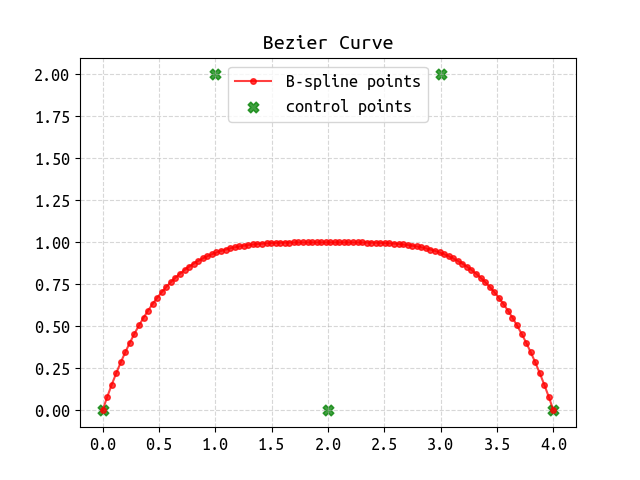
\includegraphics[width=0.9\linewidth]{../img/bezier.png}
	\caption{\normf{贝塞尔曲线}}
\end{figure}

	\subsection{\normf{B样条曲线}}
	B样条是通过一组指定点集而生成平滑曲线的柔性带。简单地说,B样条曲线就是通过控制点局部控制形状的曲线\footnote{\normf{注意是局部控制,因为其多项式的次数($k$)独立于控制点的数目($n+1$),但是有一定的限制。}}。
	
	对于$k$次\footnote{\normf{阶数等于次数加1。}}的B样条曲线,其有$n+1$个控制点、$m+1=(n+k+1)+1$个节点,即:$t_0<\dots<t_m$,且每个$t\in[t_i,t_{i+1}]$节点处的值只会由$k+1$个控制点$P_i,P_{i+1},\cdots,P_{i+k}$约束,其公式为:
	\begin{equation*}
		B_{n,k}(t)=\sum_{i=0}^{n}P_i\cdot b_{i,k}(t)
	\end{equation*}
	其中$b_{i,n}(t)$可以通过de Boor递归公式得到:
	\begin{equation*}
		\begin{aligned}
			b_{i,0}(t)&=\begin{cases}
				1\quad t_i\le t\le t_{i+1}\\
				0\quad\dots
			\end{cases}\\
		b_{i,k}(t)&=\frac{t-t_i}{t_{i+k}-t_i}b_{i,k-1}(t)+\frac{t_{i+k+1}-t}{t_{i+k+1}-t_{i+1}}b_{i+1,k-1}(t)
		\end{aligned}
	\end{equation*}
	当节点等距,称B样条为均匀。如果节点的重复度为$k+1$(即$t_0=\dots =t_k,t_{m-k}=\dots =t_m$)时,为准B样条均匀。
	\begin{figure}[htbp]
		\centering
		
		\subfigure[\normf{degree = 1}]{
			\centering
			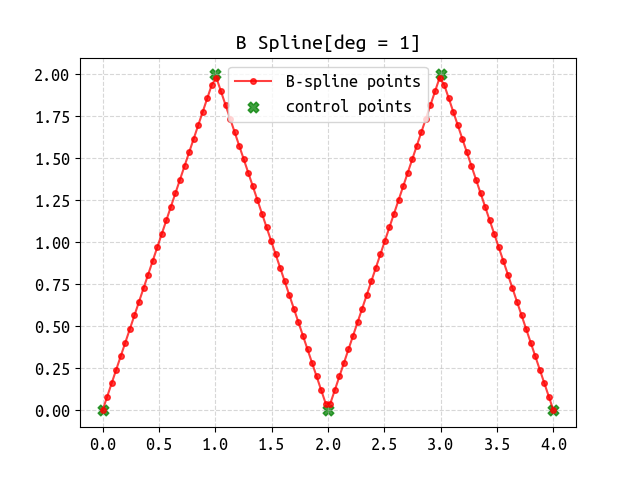
\includegraphics[width=0.45\linewidth]{../img/bspline1.png}
		}
				\subfigure[\normf{degree = 2}]{
			\centering
			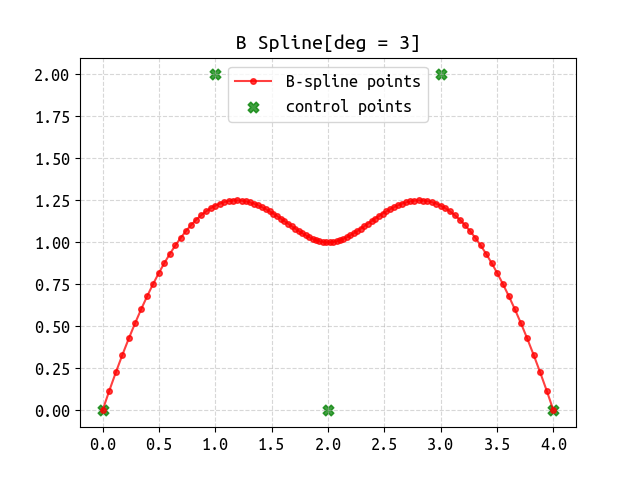
\includegraphics[width=0.45\linewidth]{../img/bspline2.png}
		}		\subfigure[\normf{degree = 3}]{
		\centering
		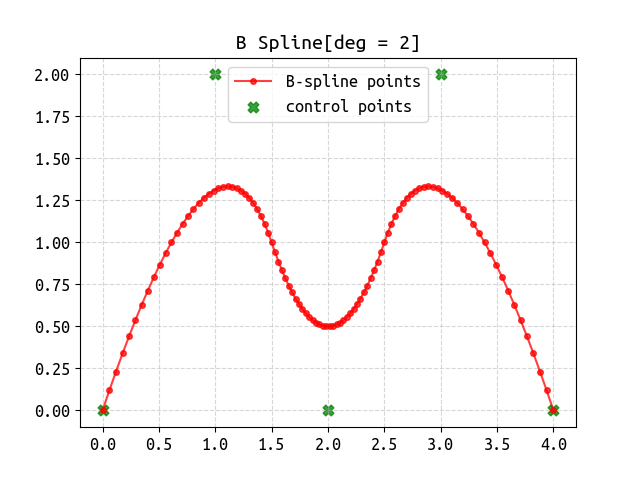
\includegraphics[width=0.45\linewidth]{../img/bspline3.png}
	}
		\caption{\normf{准B样条曲线}}
		
	\end{figure}

\section{\normf{论文算法}}
\subsection{\normf{位姿B样条}}
对于一个均匀B样条曲线,我们可以通过矩阵的形式来表达它:
\begin{equation*}
	\boldsymbol{p}(t)=\sum_{j=0}^{d}\boldsymbol{u}^T\boldsymbol{M}^{(d+1)}_{(j)}\boldsymbol{p}_{i+j}
\end{equation*}
其中$d$为该均匀B样条曲线的次,也就是说,对于$t\in [t_i,t_{i+1}]$时间范围内点点,其只会受控制点$\{ \boldsymbol{p}_i,\dots,\boldsymbol{p}_{i+d}\}$的影响,论文中选取$d=3$。公式中的向量和矩阵为:
\begin{equation*}
	\boldsymbol{M}^{(3+1)}=\frac{1}{6}\begin{pmatrix}
		1&4&1&0\\
		-3&0&3&0\\
		3&-6&3&0\\
		-1&3&-3&1
	\end{pmatrix}\quad
\boldsymbol{u}=\begin{pmatrix}
	1\\{u}\\{u}^2\\{u}^3
\end{pmatrix}
\end{equation*}
\begin{equation*}
	u=\frac{t-t_i}{t_{i+1}-t_i}
\end{equation*}
符号$\boldsymbol{M}^{(3+1)}_{(j)}$表示矩阵$\boldsymbol{M}^{(3+1)}$的第$j$列向量。通过推导,可以得到该样条曲线对时间的函数:
\begin{equation*}
	\begin{cases}
		\begin{aligned}
				\dot{\boldsymbol{p}}(t)&=\sum_{j=0}^{d}\frac{1}{t_{i+1}-t_i}\begin{pmatrix}
				0&1&2u&3u^2
			\end{pmatrix}\boldsymbol{M}^{(d+1)}_{(j)}\boldsymbol{p}_{i+j}\\
		\ddot{\boldsymbol{p}}(t)&=\sum_{j=0}^{d}\frac{1}{(t_{i+1}-t_i)^2}\begin{pmatrix}
			0&0&2&6u
		\end{pmatrix}\boldsymbol{M}^{(d+1)}_{(j)}\boldsymbol{p}_{i+j}
		\end{aligned}
	\end{cases}
\end{equation*}
	上面的B样条曲线可以描述位姿量中的平移量。
	
	对于位姿量中的旋转量,还需要进行相应的变换。不难得到,下面形式的B样条等价于上文中的公式:
	\begin{equation*}
		\boldsymbol{p}(t)=\boldsymbol{p}_i+\sum_{j=1}^{d}\boldsymbol{u}^T\tilde{\boldsymbol{M}}^{(d+1)}_{(j)}(\boldsymbol{p}_{i+j}-\boldsymbol{p}_{i+j+1})
	\end{equation*}
	d当$d=3$时,公式中矩阵$\tilde{\boldsymbol{M}}^{(3+1)}$为:
	\begin{equation*}
		\tilde{\boldsymbol{M}}^{(3+1)}=\frac{1}{6}\begin{pmatrix}
			6&5&1&0\\
			0&3&3&0\\
			0&-3&3&0\\
			0&1&-2&1
		\end{pmatrix}
	\end{equation*}
	我们利用四元素表示旋转,则有:
		\begin{equation*}
		\boldsymbol{q}(t)=\boldsymbol{q}_i\otimes \prod_{j=1}^{d}\exp(\boldsymbol{u}^T\tilde{\boldsymbol{M}}^{(d+1)}_{(j)}\log(\boldsymbol{q}_{i+j+1}^{-1}\otimes \boldsymbol{q}_{i+j})
	\end{equation*}
	其中,$\exp(\cdot)$表示从李代数到姿态流形的指数映射,而$\log(\cdot)$表示从姿态流形到李代数的对数映射,二者是相反的过程。
	
	通过对旋转B样条曲线和位移B样条曲线求时间微分,可以轻松的将其和IMU的输出角速度和线速度对应上:
	\begin{equation*}
		\begin{cases}
			\begin{aligned}
				{^{I}\boldsymbol{a}(t)}=&{^{I_0}_{I}\boldsymbol{R}^T(t)}({^{I_0}_{I}\ddot{\boldsymbol{p}}(t)}-{^{I_0}\boldsymbol{g}})\\
				{^{I}\boldsymbol{\omega}(t)}=&{^{I_0}_{I}\boldsymbol{R}^T(t)}{^{I_0}_{I}\dot{\boldsymbol{R}}(t)}
			\end{aligned}
		\end{cases}
	\end{equation*}
	其中${^{I_0}\boldsymbol{g}}$表示IMU参考帧(即第一帧)上的重力。
	\subsection{\normf{流程}}
	首先,我们可以通过IMU的输出,拟合一条姿态B样条曲线\footnote{\normf{参数其实就是得到曲线上的控制点,因为控制点确定,曲线方程就确定了。}},其最小二乘问题定义为:
	\begin{equation*}
		\boldsymbol{q}_0,\cdots,\boldsymbol{q}_N=\mathrm{min}\sum_{k=0}^{M}=\Vert {^{I_k}\boldsymbol{\omega}_m-{^{I_0}_{I}\boldsymbol{R}^T(t_k){^{I_0}_{I}\dot{\boldsymbol{R}}^T(t_k)}}\Vert}
	\end{equation*}
	其中$^{I_k}\boldsymbol{\omega}_m$为$t_k$时刻陀螺的角速度输出。注意,在优化的时候,$^{I_0}_{I}\boldsymbol{q}(t_0)$保持为单位四元素\footnote{\normf{类似与旋转矩阵中的单位矩阵,代表不旋转。}}。之后,我们就可以计算任意时刻的IMU位姿了。
	
	同时,我们基于NDT点云注册方法,进行激光里程计的估计,得到帧间的位姿变化$^{L_k}_{L_{k+1}}\boldsymbol{q}$。当然,我们可以得到在这一段时间内IMU的位姿变化$^{I_k}_{I_{k+1}}\boldsymbol{q}$。显然,这两个位姿变换之间满足:
	\begin{equation*}
		{^{I_k}_{I_{k+1}}\boldsymbol{q}}\otimes ^{I}_{L}\boldsymbol{q}=^{I}_{L}\boldsymbol{q}\otimes ^{L_k}_{L_{k+1}}\boldsymbol{q}
	\end{equation*}
	进一步,有:
	\begin{equation*}
		\alpha_k\left( \begin{bmatrix}
			{^{I_k}_{I_{k+1}}\boldsymbol{q}}
		\end{bmatrix}_L-\begin{bmatrix}
		{^{L_k}_{L_{k+1}}\boldsymbol{q}}
	\end{bmatrix}_L\right){^{I}_{L}\boldsymbol{q}}=\boldsymbol{0}
	\end{equation*}
	其中:$\left[\cdot\right]_L$表示四元素左乘积矩阵\footnote{\normf{
		假设有两个四元素$\boldsymbol{q}=\begin{pmatrix}
			q_w&\boldsymbol{q}_s^T
		\end{pmatrix}^T$、$\boldsymbol{p}=\begin{pmatrix}
		p_w&\boldsymbol{p}_s^T
	\end{pmatrix}^T$,那么$\boldsymbol{p}\otimes\boldsymbol{q}=\left[\boldsymbol{p} \right]_L\otimes\boldsymbol{q}=\left[\boldsymbol{q} \right]_R\otimes\boldsymbol{p}$
	}。其中:
		\begin{equation*}
			\left[\boldsymbol{p} \right]_L=\begin{pmatrix}
				p_w&-\boldsymbol{p}_s^T\\
				\boldsymbol{p}_s&p_w\boldsymbol{I}+\lieal[\boldsymbol{p}_s]
			\end{pmatrix}\quad 
		\left[\boldsymbol{q} \right]_R=\begin{pmatrix}
			q_w&-\boldsymbol{q}_s^T\\
			\boldsymbol{q}_s&q_w\boldsymbol{I}-\lieal[\boldsymbol{q}_s]
		\end{pmatrix}
		\end{equation*}
	},$\left[\cdot\right]_R$表示四元素右乘积矩阵。而$\alpha_k$是一个权因子:
\begin{equation*}
	\begin{cases}
		\begin{aligned}
			r_k&=\Vert 2(\arccos({^{I_k}_{I_{k+1}}q_w})-\arccos({^{L_k}_{L_{k+1}}q_w}))\\
			\alpha_k&=\begin{cases}
				\begin{aligned}
					&1\quad &r_k<threshold\\
					&\frac{threshold}{r_k}\quad &otherwise
				\end{aligned}
			\end{cases}
		\end{aligned}
	\end{cases}
\end{equation*}
所以,对于多个对应段内的姿态变换,我们可以列出方程组,求解得到激光雷达到IMU的姿态变换$^{I}_{L}\boldsymbol{q}$。至于初始化时候的IMU和激光雷达的位移量$^{I}\boldsymbol{p}_{L}$,由于加速度和重力耦合,所以不利于估计。在论文中不初始化位移量。

	初始化了IMU和LiDAR以及他们之间的姿态变换关系之后,就可以利用IMU的连续时间姿态B样条曲线对LiDAR帧进行去畸变操作,这样可以改善LiDAR的里程计精度。随后,论文将初步得到的LiDAR点云地图进行分块,然后计算每一个快内的点均值向量和方差矩阵。对于反差矩阵,可以求解得到其三个特征值:$\lambda_0\le \lambda_1\le\lambda_2$,并构造一个量来描述该块内点云的平面度(分布趋于平面的程度):
	\begin{equation*}
		\mathcal{P}=2\frac{\lambda_1-\lambda_0}{\lambda_0+\lambda_1+\lambda_2}
	\end{equation*}
	$\mathcal{P}$越接近1,越像平面。对于平面度大于阈值的平面,我们对其点云进行基于RANSAC的平面拟合,得到平面参数:$\pi=\left[\boldsymbol{n}^T,d\right]^T$。其中$\boldsymbol{n}$是平面的单位法向量,$d$是坐标原点到平面的距离。
	
	完成了初始化和LiDAR点云面片化,我们就可以进行图优化了。我们定义状态向量为:
	\begin{equation*}
		\boldsymbol{x}=\left[{^{I}_{L}\boldsymbol{q}}^T,{^{I}\boldsymbol{p}_{L}^T},\boldsymbol{x}_q^T,\boldsymbol{x}_p^T,\boldsymbol{b}_a^T,\boldsymbol{b}_g^T\right]^T
	\end{equation*}
	其中,前两个参数向量为IMU和LiDAR之间的位姿关系,后两个参数为B样条曲线的控制点位姿,最后两个为IMU的零偏误差。
	
	所以,对于一系列的LiDAR点云帧$\mathcal{L}$、加速度计的输出$\mathcal{A}$、角速度计的输出$\mathcal{W}$,可以定义一个最小二乘问题:
	\begin{equation*}
		\hat{\boldsymbol{x}}=\mathrm{min}\left\lbrace \sum_{k=\mathcal{A}}\Vert \boldsymbol{r}_a^k\Vert^2_{\boldsymbol{\Sigma}_a}+\sum_{k=\mathcal{W}}\Vert \boldsymbol{r}_\omega^k\Vert^2_{\boldsymbol{\Sigma}_\omega}+\sum_{j=\mathcal{L}}\Vert \boldsymbol{r}_l^j\Vert^2_{\boldsymbol{\Sigma}_l} \right\rbrace 
	\end{equation*}
	
	其中:
	\begin{equation*}
		\begin{aligned}
		&\begin{cases}
				\begin{aligned}
					\boldsymbol{r}_a^k&={^{I_k}\boldsymbol{a}_m}-{^{I}\boldsymbol{a}(t_k)-\boldsymbol{b}_a}\\
					\boldsymbol{r}_\omega^k&={^{I_k}\boldsymbol{\omega}_m}-{^{I}\boldsymbol{\omega}(t_k)-\boldsymbol{b}_g}
				\end{aligned}
			\end{cases}\\
		&\begin{cases}
			\begin{aligned}
				{^{L_0}\boldsymbol{p}_{L_j}}=&{^{I}_{L}\boldsymbol{R}^T}{^{I_0}_{I_j}\boldsymbol{R}}{^{I}\boldsymbol{p}_L}+{^{I}_{L}\boldsymbol{R}^T}{^{I_0}\boldsymbol{p}_{I_j}}-{^{I}_{L}\boldsymbol{R}^T}{^{I}\boldsymbol{p}_L}\\
				{^{L_0}\boldsymbol{p}_{i}}=&{^{I}_{L}\boldsymbol{R}^T}{^{I_0}_{I_j}\boldsymbol{R}}{^{I}_{L}\boldsymbol{R}}{^{L_j}\boldsymbol{p}_i}+{^{L_0}\boldsymbol{p}_{L_j}}\\
				\boldsymbol{r}_l^j=&\left[{^{L_0}\boldsymbol{p}_i}^T,1\right]\pi_j
			\end{aligned}
		\end{cases}
		\end{aligned}
	\end{equation*}
	推导:我们将第$j$帧点云里的第$i$个点${^{L_j}\boldsymbol{p}_i}$,首先推到同时刻的IMU坐标系里,然后再转到初始时刻坐标系里,最后再转回初始时刻LiDAR坐标系里,这样就相当与引入了IMU和LiDAR之间的外参。具体来说:
	\begin{equation*}
			{^{L_0}\boldsymbol{p}_{i}}={^{I}_{L}\boldsymbol{T}^{-1}}{^{I_0}_{I_j}\boldsymbol{T}}{^{I}_{L}\boldsymbol{T}}{^{L_j}\boldsymbol{p}_i}	
	\end{equation*}
	其中:
	\begin{equation*}
		{^{I}_{L}\boldsymbol{T}}=\begin{pmatrix}
			{^{I}_{L}\boldsymbol{R}}&{^{L}\boldsymbol{p}_{L}}\\
			\boldsymbol{0}&1
		\end{pmatrix}\quad {^{I}_{L}\boldsymbol{T}^{-1}}=\begin{pmatrix}
		{^{I}_{L}\boldsymbol{R}^{-1}}&-{^{I}_{L}\boldsymbol{R}^{-1}}{^{L}\boldsymbol{p}_{L}}\\
		\boldsymbol{0}&1
	\end{pmatrix}
	\end{equation*}
	通过推导可以得到上面的公式(姿态和位移分开表达)。
	
	经过批量优化之后,待估的状态就会变得更加精确。所以,之后就可以利用该状态再次进行LiDAR的点云畸变处理,而后重新优化小面片。可以通过多次迭代改善待估的状态精度。
	
	
	
\end{document}

